\documentclass[11pt,fleqn]{article}

\textheight=23.3cm
\textwidth=16.5cm
\topmargin=-15mm
\oddsidemargin=0cm

\usepackage{enumerate}
\usepackage{amsmath}
\usepackage{amssymb}
\usepackage{graphicx}
\usepackage{natbib}
\usepackage{xcolor}
\bibpunct{(}{)}{;}{a}{,}{,}
\parskip=3mm
\parindent=5mm
\baselineskip=17pt

\usepackage{hyperref}
\hypersetup{
  pdftitle={Alvarez \& Veracierto (2001) - Severance Payments in an Economy with Frictions},
  pdfauthor={Robert Kirkby},
  colorlinks=true,
  linkcolor=black,
  citecolor=black,
  urlcolor=blue,
  breaklinks=true
}

\begin{document}
\sloppy

\title{Alvarez \& Veracierto (2001) - Severance Payments in an Economy with Frictions}
\author{Robert Kirkby}
\date{\today}
\maketitle

Brief description of a replication of \cite*{AlvarezVeracierto2001}, hereafter AV2001. This is not intended as a full description of the model; rather, the goal is to show how the model is expressed in terms of the VFI Toolkit, and to record the choices we had to make where the paper is silent. For a full description see the original paper. Everything is run by \verb|AlvarezVeracierto2001.m|.

The replication covers Tables 1--5 in full. The laissez-faire economy hits every calibration target with the paper's parameters (Table \ref{tab:calibration}), and the calibrated U.S. economy of Table 1's first column replicates closely once its unemployment insurance system is calibrated, as the paper does, inside the model (Table \ref{tab:calibrationUS}). Tables 4 and 5, the unemployment insurance experiments, replicate row by row. Tables 1--3, the experiments with firing taxes, replicate in every labour market row (job-finding, layoff and unemployment rates, employment and non-search time) and in the direction of welfare, but not in the asset market: in the paper firing taxes lower the interest rate, which raises capital, and here the interest rate barely moves (Section \ref{sec:gap}). Getting there needed two corrections to the published paper, both resolved from the working-paper version \citep{AlvarezVeracierto1998}: the exit probability of establishments is $p=0.0037$, not $0.037$, and the unemployed receive no wage income (Section \ref{sec:typos}).


\section{Model description}

The model period is half a quarter, and everything is a stationary equilibrium.

\textbf{Establishments.} Output is $y=sk^\theta n^\gamma$, with $\theta=0.19$ and $\gamma=0.58$. Productivity $s\in\{0,1,\bar{s}\}$, $\bar{s}=2.12$, follows a Markov chain in which $s=0$ is absorbing (the establishment dies) and is reached with probability $p$ from either positive state, and the positive states persist with probability $\omega=0.973$. An establishment's state is $(e,s)$, where $e$ is last period's employment, and it chooses employment $n$ and capital $k$ (rented at $r=i+\delta$, $\delta=0.011$), paying a firing cost $\epsilon w^*\max[(1-\rho)e-n,0]$, where $w^*$ is the before-tax wage and $\rho=0.0031$ the retirement probability of its workers. New establishments cost $m=1950$ goods, start with $e=0$ and draw $s\in\{1,\bar{s}\}$ with equal probability. Free entry pins down $w^*$.

\textbf{Households.} A measure one of agents with utility $\sum_t\beta^t[\ln c_t + u(1-\eta_t)]$, $u(1-\eta)=\alpha[(1-\eta)^\tau-1]/\tau$, where $\eta$ is search intensity, $\beta=0.99425$, $\alpha=15.5$, $\tau=0.98$. Agents save in a riskless asset and cannot borrow. Active agents are employed or unemployed and retire with probability $\rho$; retirees survive with probability $\sigma=0.9917$ and on death are replaced by an unemployed offspring who inherits their assets (with no bequest motive). An unemployed agent who searches with intensity $\eta$ finds a job with probability $\eta^\xi$, $\xi=0.98$, at an establishment drawn from the distribution of hiring $G(e,s)$. All new hires are paid the same after-tax wage $w$ for as long as the job lasts. A worker at an establishment in state $(e,s)$ keeps the job next period with probability $\Lambda(e',s')=\min[1,n(e',s')/((1-\rho)e')]$, and a fired worker receives a one-off severance payment $\lambda w$. Employed agents and retirees do not search.

\textbf{Government.} Firing taxes and severance payments are combined in three ways: severance payments paid by the establishment to the worker ($\lambda=\epsilon$, Table 1), firing taxes rebated to establishments as an employment subsidy ($\epsilon>0$, $\lambda=0$, $w^*<w$, Tables 2 and 3), and one-off unemployment insurance financed by a payroll tax ($\lambda>0$, $\epsilon=0$, $w<w^*$, Tables 4 and 5). The budget balances every period, $0=(w^*-w)N+(\epsilon w^*-\lambda w)F$, with $N$ employment and $F$ the number of workers fired. Tables 2 and 4 make search intensity exogenous, fixed so that $\eta^\xi$ equals the average job-finding rate of the laissez-faire economy with endogenous search.

\textbf{The U.S. economy} (Table 1, first column) adds a stylised unemployment insurance system (AV2001 Section 4): a laid-off worker becomes eligible with probability 0.5; an eligible unemployed agent receives a replacement ratio of 0.66 of the wage every period and keeps eligibility with probability $\phi$ while unemployed; the benefits are financed by the firing tax $\epsilon$ (the experience-rated part) and a payroll tax; there are no severance payments. $\phi$ is chosen so that agents spend about 9 weeks collecting benefits while unemployed, and $\epsilon$ so that firing taxes finance 60\% of the benefits.


\subsection{The value function problems}

\textbf{Establishments.} The state is last period's employment $e$ and productivity $s$. Taking the interest rate $i$, the rental rate $r=i+\delta$ and the before-tax wage $w^*$ as given,
\begin{equation*}
V(e,s) = \max_{n\geq 0,\,k\geq 0} \Big\{ s k^\theta n^\gamma - w^* n - r k - \epsilon w^* \max\big[(1-\rho)e-n,\,0\big] + \frac{1}{1+i}\sum_{s'} V(n,s')\,Q(s,s') \Big\},
\end{equation*}
with $V(e,0)=-\epsilon w^*(1-\rho)e$: a dying establishment ($s=0$) fires its whole workforce, pays the firing cost once, and exits. Capital does not affect the future, so it is chosen statically, $k(s,n)=(\theta s n^\gamma/r)^{1/(1-\theta)}$, and the only dynamic choice is $n(e,s)$. Free entry requires
\begin{equation*}
m = \frac{1}{1+i}\sum_{s'\in\{1,\bar{s}\}} V(0,s')\,\psi(s').
\end{equation*}

\textbf{Households.} Let $n(e,s)$ be the establishments' employment rule, $\Lambda(e,s)=\min[1,n(e,s)/((1-\rho)e)]$ the probability of keeping a job at an establishment that starts the period in state $(e,s)$ (with $\Lambda(e,0)=0$ and $\Lambda(0,s)=0$), and $G(e,s)$ the distribution of new hires across establishment states. An employed agent with assets $a$ at an establishment in state $(e,s)$ solves
\begin{align*}
N(a,e,s) = \max_{c,\,a'\geq 0} \Big\{ \ln c &+ \beta\rho R(a') \\
&+ \beta(1-\rho)\sum_{s'} Q(s,s') \Big[ \Lambda(e',s')\,N(a',e',s') + \big(1-\Lambda(e',s')\big)\,U(a',1) \Big] \Big\} \\
\text{s.t. } \; c+a' &\leq (1+i)a + w, \qquad e'=n(e,s).
\end{align*}
An unemployed agent, $m=1$ in the period of being fired (when the severance payment $\lambda w$ arrives) and $m=0$ after, solves
\begin{align*}
U(a,m) = \max_{c,\,a'\geq 0,\,\eta\in[0,1)} \Big\{ \ln c &+ u(1-\eta) + \beta\rho R(a') \\
&+ \beta(1-\rho)\Big[ \eta^\xi \sum_{e',s'} G(e',s')\,N(a',e',s') + \big(1-\eta^\xi\big)\,U(a',0) \Big] \Big\} \\
\text{s.t. } \; c+a' &\leq (1+i)a + \lambda w\, m,
\end{align*}
and a retiree solves
\begin{equation*}
R(a) = \max_{c,\,a'\geq 0} \big\{ \ln c + \beta\sigma R(a') \big\} \quad \text{s.t. } \; c+a' \leq (1+i)a,
\end{equation*}
the value of death being zero. AV2001 write the severance payment into the assets of the newly unemployed, $U(a'+\lambda w/(1+i))$; paying it as income in the first period of unemployment is the same thing. The unemployed's budget constraint follows the working paper rather than AV2001's eq. (3.5) (Section \ref{sec:typos}). With exogenous search (Tables 2 and 4) $\eta$ is a parameter rather than a choice.

In the U.S. economy the unemployed also carry an eligibility state $b\in\{0,1\}$: $U(a,m,b)$ has income $(1+i)a+\lambda w m+\zeta w b$, with replacement ratio $\zeta=0.66$; a fired worker enters with $b=1$ with probability $\kappa=0.5$; and an eligible agent who stays unemployed keeps $b=1$ with probability $\phi$, so the continuation term $U(a',0)$ becomes $\phi\,U(a',0,1)+(1-\phi)\,U(a',0,0)$ when $b=1$ and $U(a',0,0)$ when $b=0$.


\subsection{VFI Toolkit implementation}

There are two agent problems, solved one after the other inside a root-find on the interest rate, following the algorithm of AV2001's appendix.

\textbf{Establishments} are an infinite-horizon problem, \verb|ValueFnIter_InfHorz|, with last period's employment $e$ as the endogenous state (on a 146-point grid on $[0,600]$, every integer up to 50 and coarser above), $s$ as the exogenous Markov state, and no decision variable: capital is a static choice given $(s,n)$, so it is substituted out of the return function. Their stationary distribution uses the toolkit's entry and exit (\verb|simoptions.agententryandexit=1|): entrants arrive at $e=0$, and the conditional survival probability is zero at $s=0$, so a dying establishment fires everyone and pays the firing cost for one period before leaving. The distribution is solved with a mass of entrants of one and rescaled later. The wage $w^*$ comes from \verb|fzero| on the free-entry condition.

\textbf{Households} are a second infinite-horizon problem with assets as the endogenous state. The exogenous state combines the agent's status with the state of the establishment they work at: the employed states are the establishment states $(e,s)$, $s\in\{1,\bar{s}\}$, that are reachable from entry under the establishment's policy (restricting to these is exact, and keeps the state space to between 10 and about 50 states rather than 296), followed by just-fired (with the severance payment in hand), unemployed, retired, and dead. The transition matrix is built from the establishment's policy $n(e,s)$, $\Lambda$, $G$ and the shocks. Two transition matrices are used: the value function sees an absorbing ``dead'' state with zero value, so retirees have no bequest motive, while the agent distribution sends the dead back to unemployment, since the offspring inherits the assets. With exogenous search the household has no decision variable and the exogenous state is an ordinary Markov state. With endogenous search, search intensity $\eta$ is the decision variable (51 points on $[0,0.99]$) and the exogenous state is a \emph{semi-exogenous} state (\verb|vfoptions.n_semiz|), because the unemployed's transition probabilities depend on $\eta$ through $\eta^\xi$.

In the U.S. economy the unemployed are also split by eligibility, which adds two states (just-fired eligible, receiving the first period of benefits, and unemployed eligible), and the government budget includes the benefits. $\phi$ and $\epsilon$ are calibrated by iterating between the general equilibrium solve and two updates: the time spent collecting benefits is $1/(1-c\phi)$ periods, where $c$ is the probability that an eligible agent is still unemployed next period, so $\phi$ is reset using the $c$ of the last equilibrium; and the share of benefits paid by firing taxes is proportional to $\epsilon$ given the layoffs, so $\epsilon$ is rescaled. Six iterations bring the time collecting benefits to within 0.05 weeks of 9 and the share to within half a percentage point of 60\%.

The households are solved at $w=1$: search decisions are homogeneous of degree zero in $w$ and consumption and assets of degree one, so the household side is solved once per interest rate. The scale of the establishment distribution then comes from labour market clearing (the unemployed who find jobs equal total hiring), $w$ from the government budget, and the root-find on $i$ uses goods market clearing. We check that household assets equal the value of the banks' assets, capital plus the value of establishments (eq. 3.19); they agree to within 0.5\%.

\textbf{The asset grid needs the grid interpolation layer.} Assets are on a 201-point grid on $[0.001,150]$ (wages), quadratically spaced, with the toolkit's grid interpolation layer (\verb|vfoptions.gridinterplayer=1|, 20 points between grid points, searched within 3 grid points of the coarse optimum). Without it the model is wrong in a way that does not show up as an error. In a half-quarter model the saving and dissaving flows are a few hundredths of a wage per period against a stock of about 46 wages, smaller than the grid spacing, so with pure discretization every saving decision rounds to $a'=a$: 96\% of all agents sat on a single grid point, retirees did not dissave, and the job-finding rate (which depends on how much a job is worth relative to the agent's assets) was 0.86 and moved from 0.95 to 0.67 as the grid was refined. With the interpolation layer the job-finding rate is 0.610, and it changes by at most 0.001 with 40 rather than 20 interpolation points, a search window of 2 or 5 rather than 3 grid points, 101 rather than 51 points for $\eta$, 301 rather than 201 asset points, or the top of the grid at 100 rather than 150 wages. Coarser choices move it by up to 0.003 (10 interpolation points, 26 points for $\eta$); 151 asset points are not enough (0.637). The largest share of agents at any one asset grid point is 3.4\%.


\section{Two corrections to the published paper}
\label{sec:typos}

\textbf{The exit probability is $p=0.0037$, not $0.037$.} AV2001 report $p=0.037$ (pg 488); the working paper's Table 1 has $0.0037$. Only $0.0037$ is consistent with the paper's own targets: deaths destroy 0.73\% of jobs a quarter, which is 0.37\% a half-quarter; with $p=0.037$ deaths alone give a layoff rate above the 2.9\% the paper reports, and free entry at $m=1950$ then needs establishments of more than 300 workers rather than the target of 62. With $p=0.037$ we got an average size of 312 and a layoff rate of 5.9\%; with $p=0.0037$, 63 and 2.8\%.

\textbf{The unemployed have no wage income.} AV2001's budget constraint for the unemployed (eq. 3.5) reads $c+a'\leq(1+i)a+w$. That cannot be intended: search has no benefit in consumption, so with this budget constraint nobody would search and unemployment would be absorbing. The working paper's version (its eq. 13) has $c+a'\leq(1+i)a+\lambda w$ in the period of firing and $(1+i)a$ otherwise (in the absence of the unemployment insurance of its U.S. economy), and we use that.


\section{Other choices where the paper is silent}

\begin{itemize}
\item \textbf{Measured output.} AV2001 calibrate to a capital-output ratio of 1.7 with measured output excluding the investment in new establishments (pg 488). We report output in the tables, and the capital-output ratio, on that measured basis, $Y-m\nu$, where $\nu$ is the mass of entrants.
\item \textbf{The exogenous job-finding rate} of Tables 2 and 4 is set to the average job-finding rate of our own laissez-faire economy with endogenous search, 0.610, as the paper does with its 0.61.
\item \textbf{The bottom of the asset grid} is $0.001$ wages rather than zero. An unemployed agent with no assets and no severance payment has zero consumption whatever they choose, and the resulting $-\infty$ in the value function contaminates the expectations; at $0.001$ the worst case is a small positive consumption. The borrowing constraint is otherwise unchanged.
\item \textbf{S.D. consumption} is the cross-sectional standard deviation of consumption across all agents, including retirees.
\item \textbf{Welfare} follows the paper's definition, the proportionate increase in permanent consumption that makes average lifetime utility in the laissez-faire economy equal to that in the economy under consideration. With log utility this is $\exp[(W-W_{LF})/\bar{L}]$, where $W$ is average lifetime utility and $\bar{L}$ the average expected discounted lifetime in the laissez-faire economy. ``Welfare: no search disutility'' in Tables 2 and 4 re-solves the value function with $\alpha=0$, which with exogenous search changes only a constant and not any decision.
\item \textbf{An establishment that chooses $n=0$} keeps none of its workers, $\Lambda=0$.
\item \textbf{Time collecting benefits} in the U.S. economy is the number of eligible unemployed divided by the number who become eligible each period (the average length of an eligible spell), times 6.5 weeks per period. Eligible agents receive benefits from their first period of unemployment, and lose eligibility on retirement.
\end{itemize}


\section{Results}
\label{sec:results}

Tables \ref{tab:AV2001_Table1}--\ref{tab:AV2001_Table5} show the paper's tables with ours below, numbered as in the paper, and Table \ref{tab:calibration} the calibration targets.

The U.S. column of Table 1 replicates: the job-finding rate is 53.2\% (paper 51.7\%), the layoff rate 2.8\% (2.8\%), the unemployment rate 5.6\% (5.7\%), and every index row is within 0.5 of the paper's, with welfare 99.7 (99.6). The calibrated $\phi=0.438$ and $\epsilon=0.274$ (Table \ref{tab:calibrationUS}).

Tables 4 and 5 replicate row by row: every entry is within 0.5 of the paper's, the largest differences being capital (0.5) and welfare (0.4) in the twelve-month column of Table 4. Tables 1, 2 and 3 replicate the labour market. With twelve months of severance payments (Table 1) the job-finding rate rises to 69.3\% (paper 70.5\%), the layoff rate falls to 2.0\% (2.1\%), the unemployment rate to 3.2\% (3.2\%), employment rises 1.8\% (1.7\%) and non-search time 0.6\% (0.5\%), and welfare rises to 105.5 (103.7). Table 3 is the same: job-finding 73.5\% (74.6\%), unemployment 3.1\% (3.1\%), welfare 105.6 (104.2). The one-month columns of Tables 1 and 3 show a job-finding rate a little below laissez-faire, where the paper has it a little above; the differences are a few tenths of a point.

\subsection{The gap: the interest rate does not fall}
\label{sec:gap}

The firing-tax tables differ from the paper in the asset market. In the paper (Table 2), twelve months of firing taxes lower the value of establishments, which lowers the demand for assets, so the interest rate falls from 4.0\% to 3.8\%, capital rises 0.7\%, assets fall 6.7\% and the standard deviation of consumption rises (less self-insurance). Here the interest rate falls by 0.03 points, capital falls 2.3\%, assets fall 3.5\% and the standard deviation of consumption falls. Because the welfare cost of consumption volatility is missing, welfare without search disutility falls by 3.0\% rather than 3.9\%, and welfare overall rises by 1.3 to 1.8 points more than in the paper.

We checked where the difference comes from (\verb|doPart(8)|, runs of 28 and 29 October 2026):
\begin{itemize}
\item \textbf{The establishment side replicates.} The paper's own out-of-equilibrium experiment (pg 490) holds the interest rate at its laissez-faire value and lets wages adjust to free entry; firing taxes of 3, 6 and 12 months then lower output per worker by 0.1, 0.7 and 4.3\%. We get 0.05, 0.4 and 4.1\%.
\item \textbf{The employment grid is not the cause.} On the integer grid an establishment cannot shrink by retirements alone (that needs $(1-\rho)e$ employees), so the inaction region of its $(s,S)$ rule is not representable. On a 2,063-point grid on which retirements move an establishment exactly one point down, output per worker falls by 0.2, 0.7 and 4.5\%, with layoff rates (2.7, 2.6 and 1.9\%) close to those of Table 2.
\item \textbf{The difference is in how much establishment value falls relative to the wage.} At the laissez-faire interest rate, twelve months of firing taxes lower the demand for assets per wage by only 1.2\%, and raise household savings per wage by 1.4\% (lower unemployment means more lifetime income to save for retirement). Savings per wage are very sensitive to the interest rate (39\% per percentage point of the annual rate, against $-12\%$ for asset demand), so these shifts imply the interest rate falls by 0.02 to 0.05 points (depending on the interest rate at which they are evaluated). Free entry passes most of the productivity loss on to the wage: in the twelve-month equilibrium the wage falls 3.4\% and the value of establishments 4.1\%, so household wealth per wage does not change. AV2001 report neither the wage nor the value of establishments, so we cannot tell which part of their calculation differs from ours.
\end{itemize}

Solving the laissez-faire and twelve-month equilibria of Table 2 on the 2,063-point employment grid confirms that the employment grid does not explain the gap: the interest rate falls from 4.0\% to 3.96\%, capital falls 2.5\%, assets 3.7\% and output 2.8\%, the unemployment rate falls from 4.95\% to 3.57\% and the layoff rate from 2.85\% to 1.94\%, against 2.3\%, 3.5\%, 2.6\%, 3.7\% and 2.0\% on the integer grid.

\clearpage

\section*{Tables}

\begin{table}[h!]
\caption{AV2001 Table 1: severance payments ($\lambda=\epsilon$), endogenous job-finding rate. Original (top) and replication (bottom). The U.S. column is the economy with the calibrated unemployment insurance system; all columns are relative to laissez-faire.}
\label{tab:AV2001_Table1}
\begin{center}
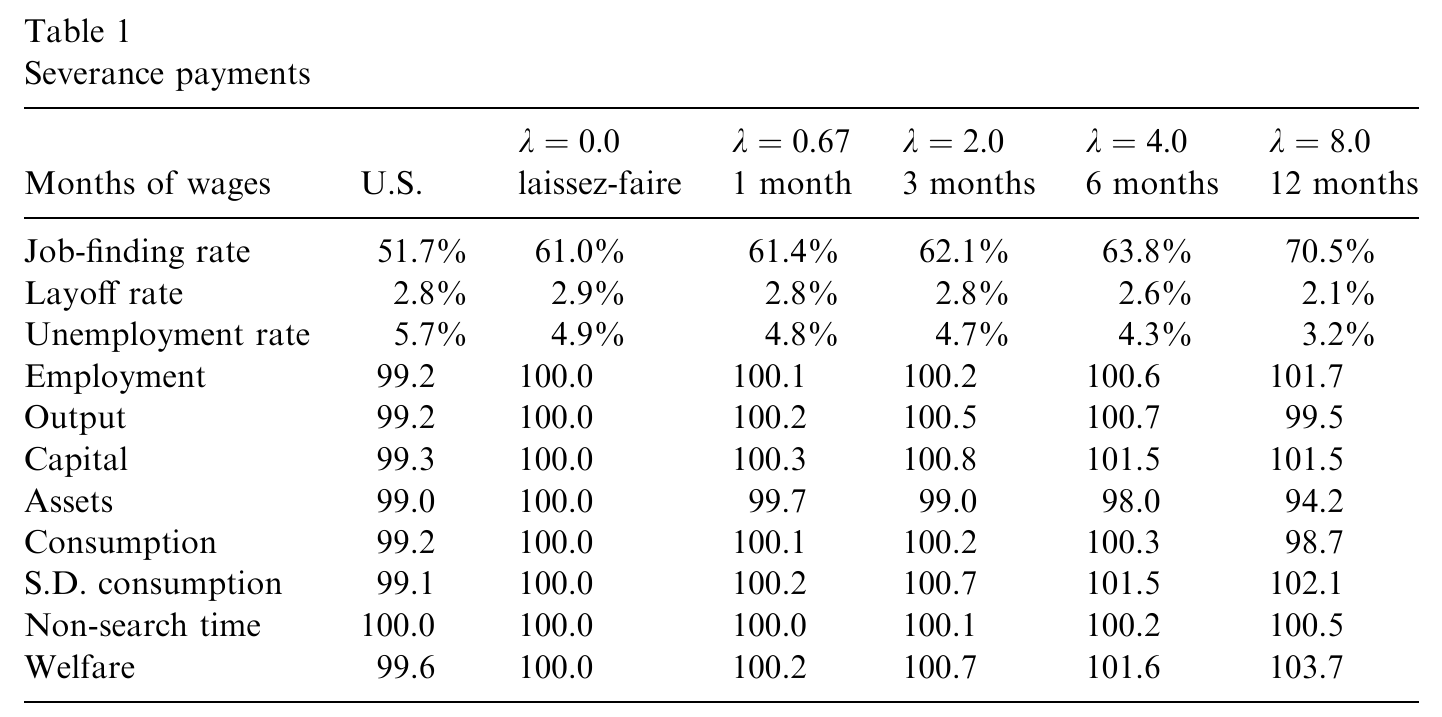
\includegraphics[width=130mm]{./OriginalTablesFigures/AV2001_Table1.png}

\vspace{3mm}
\input{../SavedOutput/LatexInputs/AV2001_Table1.tex}
\end{center}
\end{table}

\begin{table}[h!]
\caption{AV2001 Table 2: firing taxes rebated as employment subsidies, exogenous job-finding rate. Original (top) and replication (bottom).}
\label{tab:AV2001_Table2}
\begin{center}
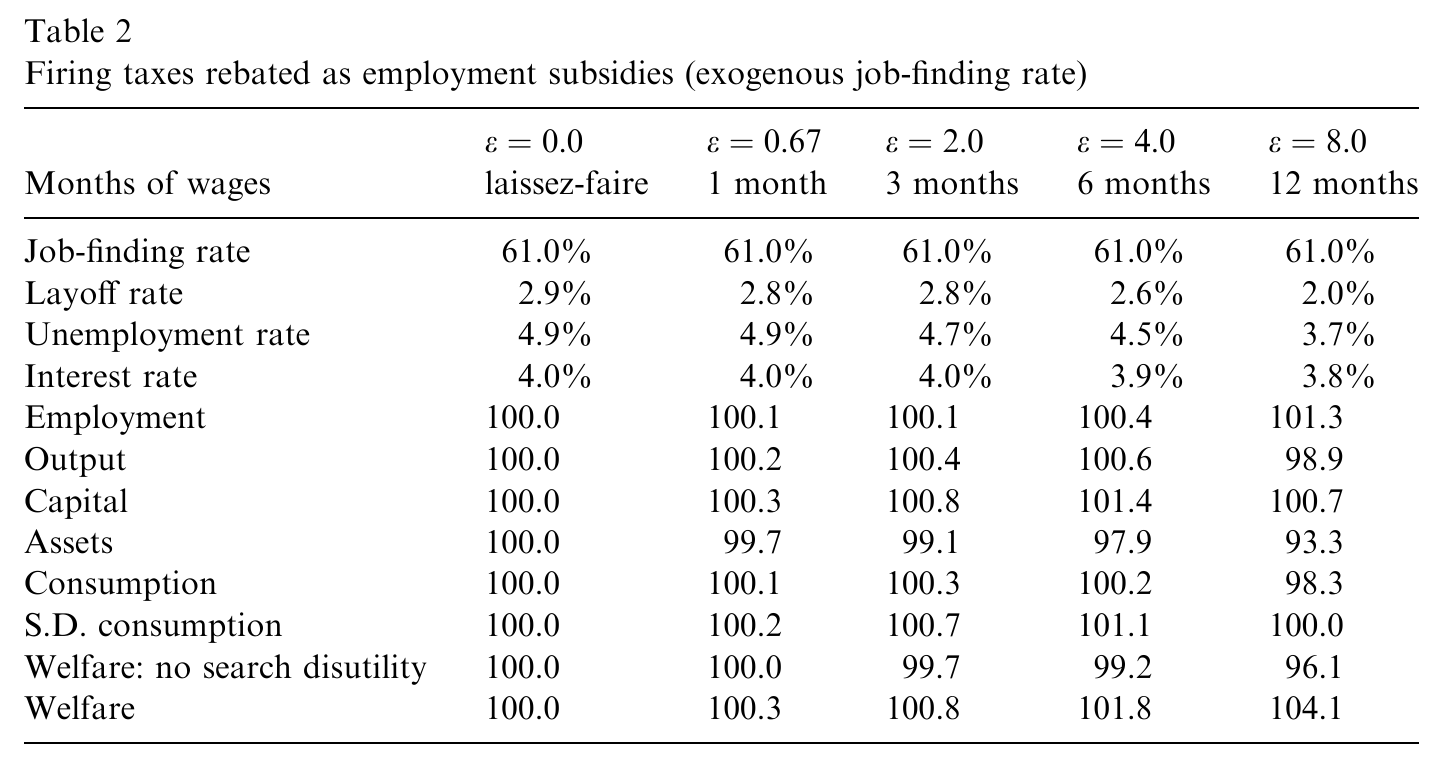
\includegraphics[width=130mm]{./OriginalTablesFigures/AV2001_Table2.png}

\vspace{3mm}
\input{../SavedOutput/LatexInputs/AV2001_Table2.tex}
\end{center}
\end{table}

\begin{table}[h!]
\caption{AV2001 Table 3: firing taxes rebated as employment subsidies, endogenous job-finding rate. Original (top) and replication (bottom).}
\label{tab:AV2001_Table3}
\begin{center}
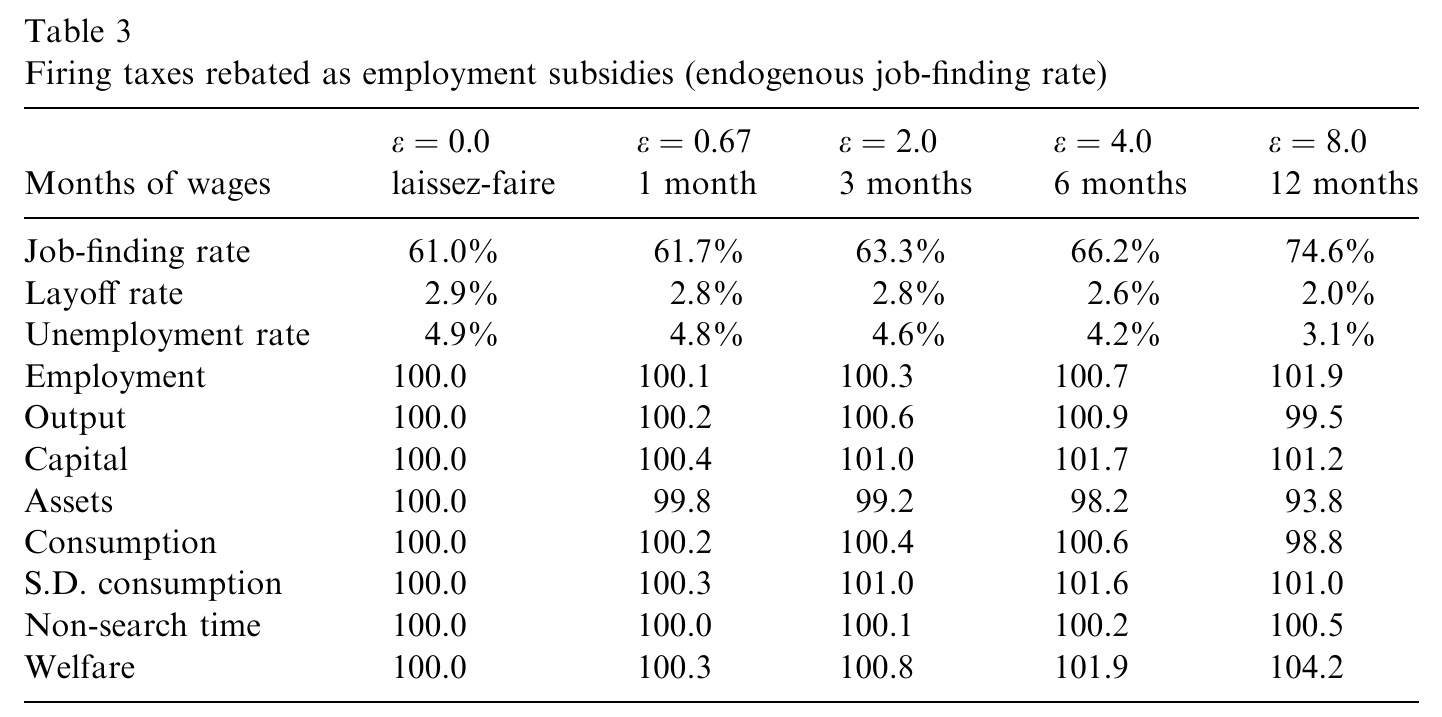
\includegraphics[width=130mm]{./OriginalTablesFigures/AV2001_Table3.png}

\vspace{3mm}
\input{../SavedOutput/LatexInputs/AV2001_Table3.tex}
\end{center}
\end{table}

\begin{table}[h!]
\caption{AV2001 Table 4: unemployment insurance paid once at layoff, financed by a payroll tax, exogenous job-finding rate. Original (top) and replication (bottom).}
\label{tab:AV2001_Table4}
\begin{center}
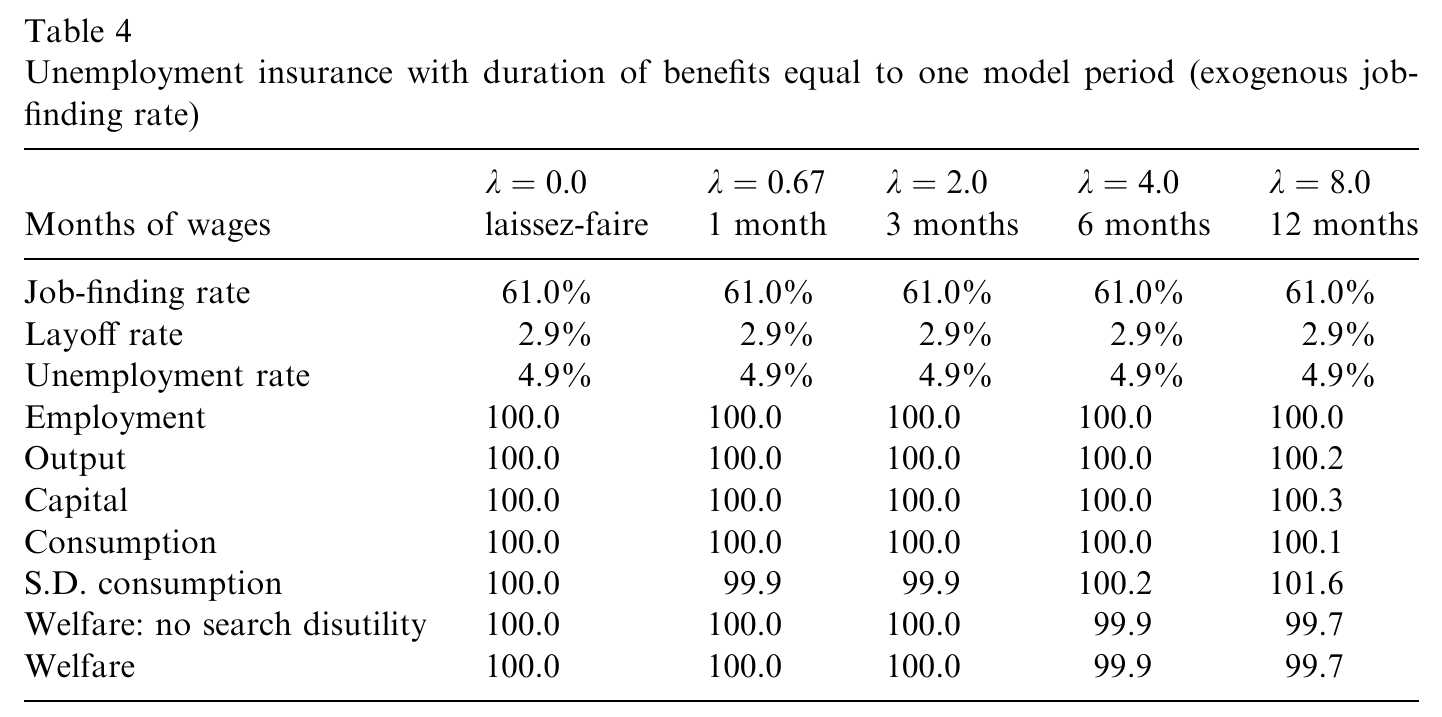
\includegraphics[width=130mm]{./OriginalTablesFigures/AV2001_Table4.png}

\vspace{3mm}
\input{../SavedOutput/LatexInputs/AV2001_Table4.tex}
\end{center}
\end{table}

\begin{table}[h!]
\caption{AV2001 Table 5: unemployment insurance paid once at layoff, financed by a payroll tax, endogenous job-finding rate. Original (top) and replication (bottom).}
\label{tab:AV2001_Table5}
\begin{center}
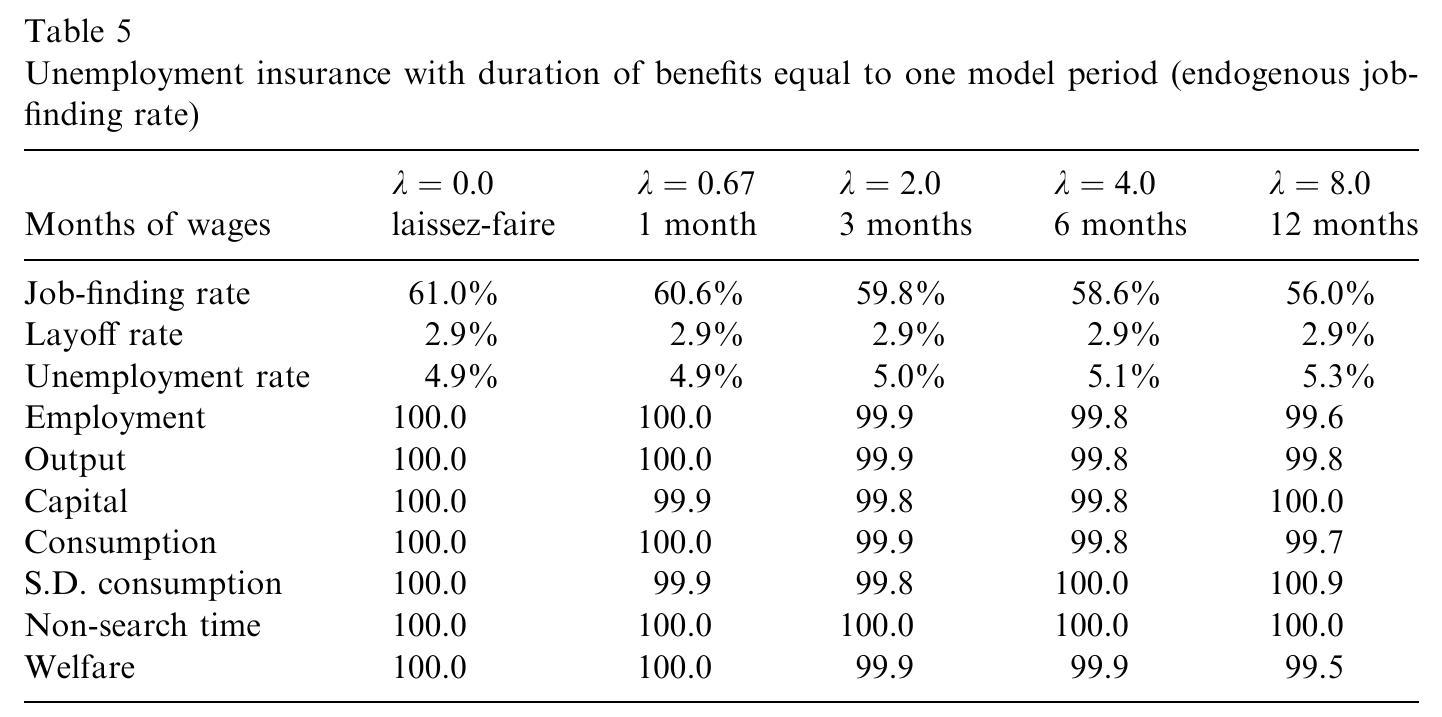
\includegraphics[width=130mm]{./OriginalTablesFigures/AV2001_Table5.png}

\vspace{3mm}
\input{../SavedOutput/LatexInputs/AV2001_Table5.tex}
\end{center}
\end{table}

\begin{table}[h!]
\caption{Calibration targets in the laissez-faire economy with endogenous search. The targets are those AV2001 state in their Section 4; the layoff and unemployment rates are their Table 1. The job-finding rate is the paper's target for an average unemployment duration of one quarter.}
\label{tab:calibration}
\begin{center}
\input{../SavedOutput/LatexInputs/AV2001_Calibration.tex}
\end{center}
\end{table}

\begin{table}[h!]
\caption{Calibration of the U.S. unemployment insurance system (Table 1, first column). The targets and the two parameters set directly are those AV2001 state in their Section 4; $\phi$ and $\epsilon$ are calibrated inside the model to the two targets.}
\label{tab:calibrationUS}
\begin{center}
\input{../SavedOutput/LatexInputs/AV2001_CalibrationUS.tex}
\end{center}
\end{table}

\clearpage

\bibliographystyle{plainnat}
\bibliography{/home/kmarshallbanana/Dropbox/RDKbiblio.bib,AV2001refs}

\end{document}
